\chapter{Advanced Simplifying Methods}\label{ch07}

\begin{tcolorbox}[colback=blue!5!white,colframe=blue!75!black]
	% Upper half of box: my "title" area
	\textcolor{blue}{\textbf{What to Expect}}
	% Lower half of the box: the content
	\tcblower
	Boolean expressions are used to describe logic circuits and by simplifying those expressions the circuits can also be simplified. This chapter introduces both the \textit{Quine-McCluskey} technique and the \textit{Karma Automated Simplification Tool}. These are methods that are useful for simplifying complex Boolean expressions that include five or more input variables. This chapter includes the following topics.
	
	\begin{itemize}
		\item Simplifying a complex Boolean expression using the Quine-McCluskey method
		\item Creating the implicants and prime implicants of a Boolean expression
		\item Combining prime implicants to create a simplified Boolean expression
		\item Simplifying a complex Boolean expression using the KARMA automated tool
	\end{itemize}
	
\end{tcolorbox}

\section{Quine-McCluskey Simplification Method}
\subsection{Introduction}

\marginpar{This method was developed by W.V. Quine and Edward J. McCluskey and is sometimes called the method of prime implicants.} When a Boolean equation involves five or more variables it becomes very difficult to solve using standard algebra techniques or Karnaugh maps; however, the Quine-McCluskey algorithm can be used to solve these types of Boolean equations.  

The Quine-McCluskey method is based upon a simple Boolean algebra principle: if two expressions differ by only a single variable and its complement then those two expressions can be combined: 

\begin{align}
	\label{ASM:eq:quine-mccluskey_combining_complements}
	ABC+ABC' &= AB 
\end{align}

The Quine-McCluskey method looks for expressions that differ by only a single variable and combines them. Then it looks at the combined expressions to find those that differ by a single variable and combines them. The process continues until there are no expressions remaining to be combined.

\subsection{Example One}
\label{ASM:subsec:quine-mccluskey_ex_1}

\subsubsection{Step 1: Create the Implicants}
\label{ASM:subsubsec:quine-mccluskey_ex_1_step_1}

Equation \ref{ASM:eq:qm_ex_1} is the Sigma representation of a Boolean equation.

\begin{align}
	\label{ASM:eq:qm_ex_1}
	\int(A,B,C,D)=\sum(0,1,2,5,6,7,9,10,11,14) 
\end{align}

Truth Table \ref{ASM:tab:qm_ex_1_minterm_table} shows the input variables for the \emph{True} minterm values.

\begin{table}[H]
	\sffamily
	\newcommand{\head}[1]{\textcolor{white}{\textbf{#1}}}		
	\begin{center}
		\rowcolors{2}{gray!10}{white} % Color every other line a light gray
		\begin{tabular}{ccccc} 
			\rowcolor{black!75}
			\head{Minterm} & \head{A} & \head{B} & \head{C} & \head{D} \\
			0 & 0 & 0 & 0 & 0 \\
			1 & 0 & 0 & 0 & 1 \\
			2 & 0 & 0 & 1 & 0 \\
			5 & 0 & 1 & 0 & 1 \\
			6 & 0 & 1 & 1 & 0 \\
			7 & 0 & 1 & 1 & 1 \\
			9 & 1 & 0 & 0 & 1 \\
			10 & 1 & 0 & 1 & 0 \\
			11 & 1 & 0 & 1 & 1 \\
			14 & 1 & 1 & 1 & 0 
		\end{tabular}
	\end{center}
	\caption{Quine-McCluskey Ex 1: Minterm Table}
  \label{ASM:tab:qm_ex_1_minterm_table}
\end{table}

To simplify this equation, the minterms that evaluate to \emph{True} (as listed above) are first placed in a minterm table so that they form sections that are easy to combine. Each section contains only the minterms that have the same number of ones. Thus, the first section contains all minterms with zero ones, the second section contains the minterms with one one, and so forth. Truth Table \ref{ASM:tab:qm_ex_1_rearranged_table} shows the minterms rearranged appropriately.

\begin{table}[H]
	\sffamily
	\newcommand{\head}[1]{\textcolor{white}{\textbf{#1}}}		
	\begin{center}
		% \rowcolors{2}{gray!10}{white} % Color every other line a light gray
		\begin{tabular}{ccc} 
			\rowcolor{black!75}
			\head{Number of 1's} & \head{Minterm} & \head{Binary} \\
			0 & 0 & 0000 \\
			\hline
			\multirow{2}{*}{1} & 1 & 0001 \\
							   & 2 & 0010 \\
			\hline
			\multirow{4}{*}{2} & 5  & 0101 \\
							   & 6  & 0110 \\		
							   & 9  & 1001 \\		
							   & 10 & 1010 \\
			\hline
			\multirow{3}{*}{3} & 7  & 0111 \\
							   & 11 & 1011 \\		
							   & 14 & 1110 \\
			\hline
		\end{tabular}
	\end{center}
	\caption{Quine-McCluskey Ex 1: Rearranged Table}
  \label{ASM:tab:qm_ex_1_rearranged_table}
\end{table}

Start combining minterms with other minterms to create Size Two Implicants (called that since each implicant combines two minterms), but only those terms that vary by a single binary digit can be combined. When two minterms are combined, the binary digit that is different between the minterms is replaced by a dash, indicating that the digit does not matter. For example, $ 0000 $ and $ 0001 $ can be combined to form $ 000- $. The table is modified to add a Size Two Implicant column that indicates all of the combined terms. Note that every minterm must be compared to every other minterm so all possible implicants are formed. This is easier than it sounds, though, since terms in section one must be compared only with section two, then those in section two are compared with section three, and so forth, since each section differs from the next by a single binary digit. The Size Two Implicant column contains the combined binary form along with the numbers of the minterms used to create that implicant. It is also important to mark all minterms that are used to create the Size Two Implicants since allowance must be made for any not combined. Therefore, in the following table, as a minterm is used it is also struck through. Table \ref{ASM:tab:quine-mccluskey_ex_1_size_2_implicants} shows the Size Two Implicants that were found.

\begin{table}[H]
	\sffamily
	\newcommand{\head}[1]{\textcolor{white}{\textbf{#1}}}		
	\begin{center}
		% \rowcolors{2}{gray!10}{white} % Color every other line a light gray
		\begin{tabular}{ccc|l} 
			\rowcolor{black!75}
			\head{1's} & \head{Mntrm} 
				& \head{Bin} & \head{Size 2} \\
			                 0 & \sout{0} & 0000 & 000- (0,1) \\
			\cline{1-3}
			\multirow{2}{*}{1} & \sout{1}  & 0001 & 00-0 (0,2) \\
			                   & \sout{2}  & 0010 & 0-01 (1,5) \\
			\cline{1-3}
			\multirow{4}{*}{2} & \sout{5}  & 0101 & -001 (1,9) \\
			                   & \sout{6}  & 0110 & 0-10 (2,6) \\		
			                   & \sout{9}  & 1001 & -010 (2,10) \\		
			                   & \sout{10} & 1010 & 01-1 (5,7) \\
			\cline{1-3}
			\multirow{3}{*}{3} & \sout{7}  & 0111 & 011- (6,7) \\
			                   & \sout{11} & 1011 & -110 (6,14) \\		
			                   & \sout{14} & 1110 & 10-1 (9,11) \\
			\cline{1-3}
			                   &    &      & 101- (10,11) \\
			                   &    &      & 1-10 (10,14) \\
			\hline
		\end{tabular}
	\end{center}
	\caption{Quine-McCluskey Ex 1: Size 2 Implicants}
  \label{ASM:tab:quine-mccluskey_ex_1_size_2_implicants}
\end{table}

All of the Size Two Implicants can now be combined to form Size Four Implicants (those that combine a total of four minterms). Again, it is essential to only combine those with only a single binary digit difference. For this step, the dash can be considered the same as a single binary digit, as long as it is in the same place for both implicants. Thus, $ -010 $ and $ -110 $ can be combined to $ --10 $, but $ -010 $ and $ 0-00 $ cannot be combined since the dash is in different places in those numbers. It helps to match up the dashes first and then look at the binary digits. Again, as the various size-two implicants are used they are marked; but notice that a single size-four implicant actually combines four size-two implicants. Table \ref{ASM:tab:quine-mccluskey_ex_1_size_4_implicants} shows the Size Four Implicants.

\begin{table}[H]
	\sffamily
	\newcommand{\head}[1]{\textcolor{white}{\textbf{#1}}}		
	\begin{center}
		% \rowcolors{2}{gray!10}{white} % Color every other line a light gray
		\begin{tabular}{ccc|l|l} 
			\rowcolor{black!75}
			\head{1's} & \head{Mntrm} 
			& \head{Bin} & \head{Size 2} & \head{Size 4} \\
			                 0 & \sout{0}  & 0000 & 000- (0,1)  & --10 (2,10,6,14) \\
			\cline{1-3}
			\multirow{2}{*}{1} & \sout{1}  & 0001 & 00-0 (0,2)  & \\
			                   & \sout{2}  & 0010 & 0-01 (1,5)  & \\
			\cline{1-3}
			\multirow{4}{*}{2} & \sout{5}  & 0101 & -001 (1,9)  & \\
                               & \sout{6}  & 0110 & \sout{0-10 (2,6)}  & \\		
			                   & \sout{9}  & 1001 & \sout{-010 (2,10)} & \\		
			                   & \sout{10} & 1010 & 01-1 (5,7)  & \\
			\cline{1-3}
			\multirow{3}{*}{3} & \sout{7}  & 0111 & 011- (6,7)  & \\
			                   & \sout{11} & 1011 & \sout{-110 (6,14)} & \\		
			                   & \sout{14} & 1110 & 10-1 (9,11) & \\
			\cline{1-3}
			                   &           &      & 101- (10,11) & \\
			                   &           &      & \sout{1-10 (10,14)} & \\
			\hline
		\end{tabular}
	\end{center}
	\caption{Quine-McCluskey Ex 1: Size 4 Implicants}
  \label{ASM:tab:quine-mccluskey_ex_1_size_4_implicants}
\end{table}

None of the terms can be combined any further. All of the minterms or implicants that are not marked are \emph{Prime Implicants}. In the table above, for example, the Size Two Implicant $ 000- $ is a Prime Implicant. The Prime Implicants will be placed in a chart and further processed in the next step. 

\subsubsection{Step 2: The Prime Implicant Table}
\label{ASM:subsubsec:quine-mccluskey_ex_1_step_2}

A \emph{Prime Implicant Table} can now be constructed, as in Table \ref{ASM:tab:qm_ex_1_prime_implicants}. The prime implicants are listed down the left side of the table, the decimal equivalent of the minterms goes across the top, and the Boolean representation of the prime implicants is listed down the right side of the table. 

\begin{table}[H]
	\sffamily
	\newcommand{\head}[1]{\textcolor{white}{\textbf{#1}}}		
	\begin{center}
		\rowcolors{2}{gray!10}{white} % Color every other line a light gray
		\begin{adjustbox}{max width=\textwidth}
		\begin{tabular}{lccccccccccc} 
			\rowcolor{black!75}
			& \head{0} & \head{1} & \head{2} & \head{5}
			& \head{6} & \head{7} & \head{9} & \head{10}
			& \head{11} & \head{14} & \\
							%      0   1   2   5   6   7   9  10  11  14  
			$ 000-\;(0,1) $       & X & X &   &   &   &   &   &   &   &   & $ A'B'C' $ \\
			$ 00-0\;(0,2) $       & X &   & X &   &   &   &   &   &   &   & $ A'B'D' $ \\
			$ 0-01\;(1,5) $       &   & X &   & X &   &   &   &   &   &   & $ A'C'D $ \\
			$ -001\;(1,9) $       &   & X &   &   &   &   & X &   &   &   & $ B'C'D $ \\
			$ 01-1\;(5,7) $       &   &   &   & X &   & X &   &   &   &   & $ A'BD $ \\
			$ 011-\;(6,7) $       &   &   &   &   & X & X &   &   &   &   & $ A'BC $ \\
			$ 10-1\;(9,11) $      &   &   &   &   &   &   & X &   & X &   & $ AB'D $ \\
			$ 101-\;(10,11) $     &   &   &   &   &   &   &   & X & X &   & $ AB'C $ \\
			$ --10\;(2,10,6,14) $ &   &   & X &   & X &   &   & X &   & X & $ CD' $ \\
			\hline
		\end{tabular}
		\end{adjustbox}
	\end{center}
	\caption{Quine-McCluskey Ex 1: Prime Implicants}
  \label{ASM:tab:qm_ex_1_prime_implicants}
\end{table}

An \emph{X} marks the intersection where each minterm (on the top row) is used to form one of the prime implicants (in the left column). Thus, minterm $ 0 $ (or $ 0000 $) is used to form the prime implicant $ 000- (0,1) $ in row one and $ 00-0 (0,2) $ in row two. 

The Essential Prime Implicants can be found by looking for columns that contain only one \emph{X}. The column for minterm $ 14 $ has only one \emph{X}, in the last row, $ --10 (2,10,6,14) $; thus, it is an Essential Prime Implicant. That means that the term in the right column for the last row, $ CD' $, must appear in the final simplified equation. However, that term also covers the columns for $ 2 $, $ 6 $, and $ 10 $; so they can be removed from the table. The Prime Implicant table is then simplified to \ref{ASM:tab:qm_ex_1_1st_iteration}.

\begin{table}[H]
	\sffamily
	\newcommand{\head}[1]{\textcolor{white}{\textbf{#1}}}		
	\begin{center}
		\rowcolors{2}{gray!10}{white} % Color every other line a light gray
		\begin{adjustbox}{max width=\textwidth}
			\begin{tabular}{lccccccc} 
				\rowcolor{black!75}
				& \head{0} & \head{1} & \head{5}
				& \head{7} & \head{9} & \head{11} & \\
				%                      0   1   5   7   9  11   
				$ 000-\;(0,1) $       & X & X &   &   &   &   & $ A'B'C' $ \\
				$ 00-0\;(0,2) $       & X &   &   &   &   &   & $ A'B'D' $ \\
				$ 0-01\;(1,5) $       &   & X & X &   &   &   & $ A'C'D $ \\
				$ -001\;(1,9) $       &   & X &   &   & X &   & $ B'C'D $ \\
				$ 01-1\;(5,7) $       &   &   & X & X &   &   & $ A'BD $ \\
				$ 011-\;(6,7) $       &   &   &   & X &   &   & $ A'BC $ \\
				$ 10-1\;(9,11) $      &   &   &   &   & X & X & $ AB'D $ \\
				$ 101-\;(10,11) $     &   &   &   &   &   & X & $ AB'C $ \\
				\hline
			\end{tabular}
		\end{adjustbox}
	\end{center}
	\caption{Quine-McCluskey Ex 1: 1st Iteration}
  \label{ASM:tab:qm_ex_1_1st_iteration}
\end{table}

The various rows can now be combined in any order the designer desires. For example, if row $ 10-1 (9,11) $, is selected as a required implicant in the solution, then minterms $ 9 $ and $ 11 $ are accounted for in the final equation, which means that all \emph{X} marked in those columns can be removed. When that is done, then, rows $ 101- (10,11) $ and $ 10-1 (9,11) $ no longer have any marks in the table, and they can be removed. Table \ref{ASM:tab:qm_ex_1_2nd_iteration} shows the last iteration of this solution. 

\begin{table}[H]
	\sffamily
	\newcommand{\head}[1]{\textcolor{white}{\textbf{#1}}}		
	\begin{center}
		\rowcolors{2}{gray!10}{white} % Color every other line a light gray
		\begin{adjustbox}{max width=\textwidth}
			\begin{tabular}{lccccccc} 
				\rowcolor{black!75}
				& \head{0} & \head{1} & \head{5}
				& \head{7} & \\
				%                      0   1   5   7      
				$ 000-\;(0,1) $       & X & X &   &   & $ A'B'C' $ \\
				$ 00-0\;(0,2) $       & X &   &   &   & $ A'B'D' $ \\
				$ 0-01\;(1,5) $       &   & X & X &   & $ A'C'D $ \\
				$ -001\;(1,9) $       &   & X &   &   & $ B'C'D $ \\
				$ 01-1\;(5,7) $       &   &   & X & X & $ A'BD $ \\
				$ 011-\;(6,7) $       &   &   &   & X & $ A'BC $ \\
				\hline
			\end{tabular}
		\end{adjustbox}
	\end{center}
	\caption{Quine-McCluskey Ex 1: 2nd Iteration}
  \label{ASM:tab:qm_ex_1_2nd_iteration}
\end{table}

The designer next decided to select $ 01-1 (5,7) $, $ A'BD $, as a required implicant. That will include minterms $ 5 $ and $ 7 $, and those columns may be removed along with rows $ 01-1 (5,7) $, $ A'BD $, and $ 011- (6,7) $, $ A'BC $, as shown in Table \ref{ASM:tab:qm_ex_1_3rd_iteration}.

\begin{table}[H]
	\sffamily
	\newcommand{\head}[1]{\textcolor{white}{\textbf{#1}}}		
	\begin{center}
		\rowcolors{2}{gray!10}{white} % Color every other line a light gray
		\begin{adjustbox}{max width=\textwidth}
			\begin{tabular}{lccccccc} 
				\rowcolor{black!75}
				& \head{0} & \head{1} & \\
				%                       0   1         
				$ 000-\;(0,1) $       & X & X & $ A'B'C' $ \\
				$ 00-0\;(0,2) $       & X &   & $ A'B'D' $ \\
				$ 0-01\;(1,5) $       &   & X & $ A'C'D $ \\
				$ -001\;(1,9) $       &   & X & $ B'C'D $ \\
				\hline
			\end{tabular}
		\end{adjustbox}
	\end{center}
	\caption{Quine-McCluskey Ex 1: 3rd Iteration}
  \label{ASM:tab:qm_ex_1_3rd_iteration}
\end{table}

The last two minterms ($ 0 $ and $ 1 $) can be covered by the implicant $ 000- (0,1) $, and that also eliminates the last three rows in the chart. 

The original Boolean expression, then, has been simplified from ten minterms to Equation \ref{ASM:eq:qm_ex_1_solution}.

\begin{align}
	\label{ASM:eq:qm_ex_1_solution}
	A'B'C'+A'BD+AB'D+CD' = Y 
\end{align}

\subsection{Example Two}
\label{ASM:subsec:quine-mccluskey_ex_2}

\subsubsection{Step 1: Create the Implicants}
\label{ASM:subsubsec:quine-mccluskey_ex_2_step_1}

Given Equation \ref{ASM:eq:qm_ex_2}, which is a Sigma representation of a Boolean equation.

\begin{align}
\label{ASM:eq:qm_ex_2}
\int(A,B,C,D,E,F)=\sum(0,1,8,9,12,13,14,15,32,33,37,39,48,56) 
\end{align}

Truth Table \ref{ASM:tab:qm_ex_2_minterm_table} shows the \emph{True} minterm values.

\begin{table}[H]
	\sffamily
	\newcommand{\head}[1]{\textcolor{white}{\textbf{#1}}}		
	\begin{center}
		\rowcolors{2}{gray!10}{white} % Color every other line a light gray
		\begin{tabular}{ccccccc} 
			\rowcolor{black!75}
			\head{Minterm} & \head{A} & \head{B} & \head{C} 
				& \head{D} & \head{E} & \head{F} \\
			0  & 0 & 0 & 0 & 0 & 0 & 0 \\
			1  & 0 & 0 & 0 & 0 & 0 & 1 \\
			8  & 0 & 0 & 1 & 0 & 0 & 0 \\
			9  & 0 & 0 & 1 & 0 & 0 & 1 \\
			12 & 0 & 0 & 1 & 1 & 0 & 0 \\
			13 & 0 & 0 & 1 & 1 & 0 & 1 \\
			14 & 0 & 0 & 1 & 1 & 1 & 0 \\
			15 & 0 & 0 & 1 & 1 & 1 & 1 \\
			32 & 1 & 0 & 0 & 0 & 0 & 0 \\
			33 & 1 & 0 & 0 & 0 & 0 & 1 \\
			37 & 1 & 0 & 0 & 1 & 0 & 1 \\
			39 & 1 & 0 & 0 & 1 & 1 & 1 \\
			48 & 1 & 1 & 0 & 0 & 0 & 0 \\
			56 & 1 & 1 & 1 & 0 & 0 & 0 \\
		\end{tabular}
	\end{center}
	\caption{Quine-McCluskey Ex 2: Minterm Table}
  \label{ASM:tab:qm_ex_2_minterm_table}
\end{table}

To simplify this equation, the minterms that evaluate to \emph{True} are placed in a minterm table so that they form sections that are easy to combine. Each section contains only the minterms that have the same number of ones. Thus, the first section contains all minterms with zero ones, the second section contains the minterms with one one, and so forth. Table \ref{ASM:tab:qm_ex_2_rearranged_table} shows the rearranged truth table.

\begin{table}[H]
	\sffamily
	\newcommand{\head}[1]{\textcolor{white}{\textbf{#1}}}		
	\begin{center}
		% \rowcolors{2}{gray!10}{white} % Color every other line a light gray
		\begin{tabular}{ccc} 
			\rowcolor{black!75}
			\head{Number of 1's} & \head{Minterm} & \head{Binary} \\
							 0 & 0  & 000000 \\
			\hline
			\multirow{3}{*}{1} & 1  & 000001 \\
                               & 8  & 001000 \\
                               & 32 & 100000 \\
 			\hline
			\multirow{4}{*}{2} & 9  & 001001 \\
                               & 12 & 001100 \\		
							   & 33 & 100001 \\		
							   & 48 & 110000 \\
			\hline
			\multirow{3}{*}{3} & 13 & 001101 \\
							   & 14 & 001110 \\		
							   & 37 & 100101 \\		
							   & 56 & 111000 \\
			\hline
			\multirow{2}{*}{4} & 15 & 001111 \\
							   & 39 & 100111 \\		
			\hline
		\end{tabular}
	\end{center}
	\caption{Quine-McCluskey Ex 2: Rearranged Table}
  \label{ASM:tab:qm_ex_2_rearranged_table}
\end{table}

Start combining minterms with other minterms to create Size Two Implicants, as in Table \ref{ASM:tab:qm_ex_2_size_2_implicants}.

\begin{table}[H]
	\sffamily
	\newcommand{\head}[1]{\textcolor{white}{\textbf{#1}}}		
	\begin{center}
		% \rowcolors{2}{gray!10}{white} % Color every other line a light gray
		\begin{tabular}{ccc|c} 
			\rowcolor{black!75}
			\head{1's} & \head{Mntrm} & \head{Bin} & \head{Size 2} \\
							 0 & \sout{0} & 000000 & 00000- (0,1) \\
			\cline{1-3}
			\multirow{3}{*}{1} & \sout{1}  & 000001 & -000000 (0,32) \\
							   & \sout{8}  & 001000 & 00-000 (0,8) \\
							   & \sout{32} & 100000 & -00001 (1,33) \\
			\cline{1-3}
			\multirow{4}{*}{2} & \sout{9}  & 001001 & 00-001 (1,9) \\
							   & \sout{12} & 001100 & 10000- (32,33) \\		
				  			   & \sout{33} & 100001 & 1-0000 (32,48) \\		
							   & \sout{48} & 110000 & 00100- (8,9) \\
			\cline{1-3}
			\multirow{3}{*}{3} & \sout{13} & 001101 & 001-00 (8,12) \\
							   & \sout{14} & 001110 & 100-01 (33,37) \\		
							   & \sout{37} & 100101 & 001-01 (9,13) \\		
						       & \sout{56} & 111000 & 00110- (12,13) \\
			\cline{1-3}
			\multirow{2}{*}{4} & \sout{15} & 001111 & 0011-0 (12,14) \\
							   & \sout{39} & 100111 & 11-000 (48,56) \\		
							   &    &        & 1001-1 (37,39) \\		
							   &    &        & 0011-1 (13,15) \\		
							   &    &        & 00111- (14,15) \\		
			\hline
		\end{tabular}
	\end{center}
	\caption{Quine-McCluskey Ex 2: Size Two Implicants}
  \label{ASM:tab:qm_ex_2_size_2_implicants}
\end{table}

All of the Size Two Implicants can now be combined to form Size Four Implicants, as in Table \ref{ASM:tab:qm_ex_2_size_4_implicants}.

\begin{table}[H]
	\sffamily
	\newcommand{\head}[1]{\textcolor{white}{\textbf{#1}}}		
	\begin{center}
		% \rowcolors{2}{gray!10}{white} % Color every other line a light gray
		\begin{tabular}{ccc|c|c} 
			\rowcolor{black!75}
			\head{1's} & \head{Mntrm} & \head{Bin} 
				& \head{Size 2} & \head{Size 4} \\
							  0 & \sout{0} & 000000 & \sout{00000- (0,1)}   & -0000- (0,1,32,33) \\
			\cline{1-3}
			\multirow{3}{*}{1} & \sout{1}  & 000001 & \sout{-000000 (0,32)} & 00-00- (0,1,8,9)\\
							   & \sout{8}  & 001000 & \sout{00-000 (0,8)}   & 001-0- (8,9,12,13)\\
						       & \sout{32} & 100000 & \sout{-00001 (1,33)}  & 0011-- (12,13,14,15)\\
			\cline{1-3}
			\multirow{4}{*}{2} & \sout{9}  & 001001 & \sout{00-001 (1,9)}   & \\
							   & \sout{12} & 001100 & \sout{10000- (32,33)} & \\		
							   & \sout{33} & 100001 & 1-0000 (32,48)        & \\		
							   & \sout{48} & 110000 & \sout{00100- (8,9)}   & \\
			\cline{1-3}
			\multirow{3}{*}{3} & \sout{13} & 001101 & \sout{001-00 (8,12)}  & \\
							   & \sout{14} & 001110 & 100-01 (33,37)        & \\		
							   & \sout{37} & 100101 & \sout{001-01 (9,13)}  & \\		
							   & \sout{56} & 111000 & \sout{00110- (12,13)} & \\
			\cline{1-3}
			\multirow{2}{*}{4} & \sout{15} & 001111 & \sout{0011-0 (12,14)} & \\
							   & \sout{39} & 100111 & 11-000 (48,56)        & \\		
							   &    &        & 1001-1 (37,39) 		        & \\		
							   &    &        & \sout{0011-1 (13,15)}	    & \\		
							   &    &        & \sout{00111- (14,15)} 	    & \\		
			\hline
		\end{tabular}
	\end{center}
	\caption{Quine-McCluskey Ex 2: Size 4 Implicants}
  \label{ASM:tab:qm_ex_2_size_4_implicants}
\end{table}

None of the terms can be combined any further. All of the minterms or implicants that are not struck through are \emph{Prime Implicants}. In the table above, for example, $ 1-0000 $ is a Prime Implicant. The Prime Implicants are next placed in a table and further processed. 

\subsubsection{Step 2: The Prime Implicant Table}
\label{ASM:subsubsec:quine-mccluskey_ex_2_step_2}

A \emph{Prime Implicant Table} can now be constructed, as in Table \ref{ASM:tab:qm_ex_2_prime_implicants}. The prime implicants are listed down the left side of the table, the decimal equivalent of the minterms goes across the top, and the Boolean representation of the prime implicants is listed down the right side of the table. 

\begin{table}[H]
	\sffamily
	\newcommand{\head}[1]{\textcolor{white}{\textbf{#1}}}		
	\begin{center}
		\rowcolors{2}{gray!10}{white} % Color every other line a light gray
		\begin{adjustbox}{max width=\textwidth}
			\begin{tabular}{lccccccccccccccc} 
				\rowcolor{black!75}
				& \head{0} & \head{1} & \head{8} & \head{9}
				& \head{12} & \head{13} & \head{14} & \head{15}
				& \head{32} & \head{33} & \head{37} & \head{39} 
				& \head{48} & \head{56} & \\
				%      			            0   1   8   9  12  13  14  15  32  33  37  39  48  56
				$ 11-000\;(48,56) $       &   &   &   &   &   &   &   &   &   &   &   &   & X & X & $ ABD'D'F' $ \\
				$ 00-00-\;(0,1,8,9) $     & X & X & X & X &   &   &   &   &   &   &   &   &   &   & $ A'B'D'E' $ \\
				$ 1001-1\;(37,39) $       &   &   &   &   &   &   &   &   &   &   & X & X &   &   & $ AB'C'DF $ \\
				$ 1-0000\;(32,48) $       &   &   &   &   &   &   &   &   & X &   &   &   & X &   & $ AC'D'E'F' $ \\
				$ 0011--\;(12,13,14,15) $ &   &   &   &   & X & X & X & X &   &   &   &   &   &   & $ A'B'CD $ \\
				$ -0000-\;(0,1,32,33) $   & X & X &   &   &   &   &   &   & X & X &   &   &   &   & $ B'C'D'E' $ \\
				$ 001-0-\;(8,9,12,13) $   &   &   & X & X & X & X &   &   &   &   &   &   &   &   & $ A'B'CE' $ \\
				$ 100-01\;(33,37) $       &   &   &   &   &   &   &   &   &   & X & X &   &   &   & $ AB'C'E'F $ \\
				\hline
			\end{tabular}
		\end{adjustbox}
	\end{center}
	\caption{Quine-McCluskey Ex 2: Prime Implicants}
  \label{ASM:tab:qm_ex_2_prime_implicants}
\end{table}

In the above table, there are four columns that contain only one \emph{X}: $ 14 $, $ 15 $, $ 39 $, and $ 56 $. The rows that intersect the columns at that mark are \emph{Essential Prime Inplicants}, and their Boolean Expressions must appear in the final equation. Therefore, the final equation will contain, at a minimum: $ A'B'CD $ (row $ 5 $, covers minterms $ 14 $ and $ 15 $), $ AB'C'DF $ (row $ 3 $, covers minterm $ 39 $), and $ ABD'E'F' $ (row $ 1 $, covers minterm $ 56 $). Since those expressions are in the final equation, the rows that contain those expressions can be removed from the chart in order to make further analysis less confusing. 

Also, because the rows with Essential Prime Implicants are contained in the final equation, other minterms marked by those rows are covered and need no further consideration. For example, minterm $ 48 $ is covered by row one (used for minterm $ 56 $), so column $ 48 $ can be removed from the table. In a similar fashion, columns $ 12 $, $ 13 $, and $ 37 $ are covered by other minterms, so they can be removed from the table. Table \ref{ASM:tab:qm_ex_2_1st_iteration} shows the next iteration of this process.

\begin{table}[H]
	\sffamily
	\newcommand{\head}[1]{\textcolor{white}{\textbf{#1}}}		
	\begin{center}
		\rowcolors{2}{gray!10}{white} % Color every other line a light gray
		\begin{adjustbox}{max width=\textwidth}
			\begin{tabular}{lccccccc} 
				\rowcolor{black!75}
				& \head{0} & \head{1} & \head{8} & \head{9}
				& \head{32} & \head{33} & \\
				%      			            0   1   8   9  32  33 
				$ 00-00-\;(0,1,8,9) $     & X & X & X & X &   &   & $ A'B'D'E' $ \\
				$ 1-0000\;(32,48) $       &   &   &   &   & X &   & $ AC'D'E'F' $ \\
				$ -0000-\;(0,1,32,33) $   & X & X &   &   & X & X & $ B'C'D'E' $ \\
				$ 001-0-\;(8,9,12,13) $   &   &   & X & X &   &   & $ A'B'CE' $ \\
				$ 100-01\;(33,37) $       &   &   &   &   &   & X & $ AB'C'E'F $ \\
				\hline
			\end{tabular}
		\end{adjustbox}
	\end{center}
	\caption{Quine-McCluskey Ex 2: 1st Iteration}
  \label{ASM:tab:qm_ex_2_1st_iteration}
\end{table}

The circuit designer can select the next term to include in the final equation from any of the five rows still remaining in the chart; however, the first term ($ 00-00- $, or $ A'B'D'E' $) would eliminate four columns, so that would be a logical next choice. When that term is selected for the final equation, then row one, $ 00-00- $, can be removed from the chart; and columns $ 0 $, $ 1 $, $ 8 $, and $ 9 $ can be removed since those minterms are covered. 

The minterms marked for row $ 001-0- (8,9,12,13) $ are also covered, so this row can be removed. Table \ref{ASM:tab:qm_ex_2_2nd_iteration} shows the next iteration.

\begin{table}[H]
	\sffamily
	\newcommand{\head}[1]{\textcolor{white}{\textbf{#1}}}		
	\begin{center}
		\rowcolors{2}{gray!10}{white} % Color every other line a light gray
		\begin{adjustbox}{max width=\textwidth}
			\begin{tabular}{lccc} 
				\rowcolor{black!75}
				& \head{32} & \head{33} & \\
				%      			           32  33 
				$ 1-0000\;(32,48) $       & X &   & $ AC'D'E'F' $ \\
				$ -0000-\;(0,1,32,33) $   & X & X & $ B'C'D'E' $ \\
				$ 100-01\;(33,37) $       &   & X & $ AB'C'E'F $ \\
				\hline
			\end{tabular}
		\end{adjustbox}
	\end{center}
	\caption{Quine-McCluskey Ex 2: 2nd Iteration}
  \label{ASM:tab:qm_ex_2_2nd_iteration}
\end{table}

For the next simplification, row $ -0000- $ is selected since that would also cover the minterms that are marked for all remaining rows. Thus, the expression $ B'C'D'E' $ will become part of the final equation. 

When the analysis is completed, the original equation (\ref{ASM:eq:qm_ex_2}), which contained $ 14 $ minterms, is simplified into Equation \ref{ASM:eq:qm_ex_2_solution}, which contains only five terms.

\begin{align}
	\label{ASM:eq:qm_ex_2_solution}
	ABD'E'F'+A'B'D'E'+AB'C'DF+A'B'CD+B'C'D'E' = Y 
\end{align}

\subsection{Summary}
\label{ASM:subsec:quine-mccluskey_summary}

While the Quine–McCluskey method is useful for large Boolean expressions containing multiple inputs, it is also tedious and prone to error when done by hand. Also, there are some Boolean expressions (called ``Cyclic'' and ``Semi-Cyclic'' Primes) that do not reduce using this method. Finally, both Karnaugh maps and Quine-McCluskey methods become very complex when more than one output is required of a circuit. Fortunately, many automated tools are available to simplify Boolean expressions using advanced mathematical techniques. 

\subsection{Practice Problems}
\label{ASM:subsec:quine-mccluskey_practice_problems}

The following problems are presented as practice for using the Quine-McClusky method to simplify a Boolean expression. Note: designers can select different Prime Implicants so the simplified expression could vary from what is presented below. 

\begin{table}[H]
	\sffamily
	\begin{center}
		\begin{tabular}{c c p{6cm} }
			\multirow{2}{*}{\textbf{1}} 
			& Expression & $ \int(A,B,C,D) = \sum(0,1,2,5,6,7,9,10,11,14) $ \\
			& \cellcolor{gray!10} Simplified 
			& \cellcolor{gray!10} $ A'B'C'+A'BD+AB'D+CD' $ \\
			\hline
			\multirow{2}{*}{\textbf{2}} 
			& Exression & $ \int(A,B,C,D) = \sum(0,1,2,3,6,7,8,9,14,15) $ \\
			& \cellcolor{gray!10} Simplified 
			& \cellcolor{gray!10} $ A'C+BC+B'C' $ \\
			\hline
			\multirow{2}{*}{\textbf{3}} 
			& Exression & $ \int(A,B,C,D) = \sum(1,5,7,8,9,10,11,13,15) $ \\
			& \cellcolor{gray!10} Simplified 
			& \cellcolor{gray!10} $ C'D+AB'+BD $ \\
			\hline
			\multirow{2}{*}{\textbf{3}} 
			& Exression & $ \int(A,B,C,D,E) = \sum(0,4,8,9,10,11,12,13,14,15,16,20,24,28) $ \\
			& \cellcolor{gray!10} Simplified 
			& \cellcolor{gray!10} $ A'B+D'E' $ \\
		\end{tabular}
	\end{center}
	\caption{Quine-McCluskey Practice Problems}
  \label{ASM:tab:quine-mccluskey_practice_problems}
\end{table}

%***************************************************************************
% Section: Automated Tools
%***************************************************************************
\clearpage\section{Automated Tools}
\label{ASM:sec:automated_tools}

\subsection{KARMA}
\label{ASM:subsec:introduction_to_automated_tools}

There are numerous automated tools available to aid in simplifying complex Boolean equations. Many of the tools are quite expensive and intended for professionals working full time in large companies; but others are inexpensive, or even free of charge, and are more than adequate for student use. One free tool, a Java application named \gls{karma}, can be downloaded from \url{http://bit.ly/2mcXVp9} and installed on a local computer, though the website also has a free online version that can be used without installation. \Gls{karma} helps to simplify complex Boolean expressions using both Karnaugh Maps and Quine-McCluskey methods. \Gls{karma} is a good program with numerous benefits.

When first started, \gls{karma} looks like Figure \ref{fig:07_01}. 

\begin{figure}[H]
	\centering
	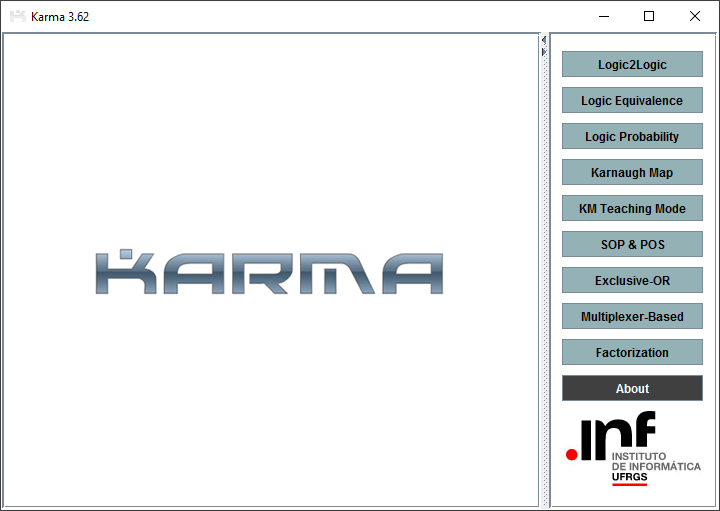
\includegraphics[width=\maxwidth{.95\linewidth}]{gfx/07_01}
	\caption{KARMA Start Screen}
	\label{fig:07_01}
\end{figure}

The right side of the screen contains a row of tools available in \gls{karma} and the main part of the screen is a canvas where most of the work is done. The following tools are available:

\begin{itemize}
	\item \textbf{Logic2Logic}. Converts between two different logical representations of data; for example, a Truth Table can be converted to Boolean expressions.

	\item \textbf{Logic Equivalence}. Compares two functions and determines if they are equivalent; for example, a truth table can be compared with a SOP expression to see if they are the same.

	\item \textbf{Logic Probability}. Calculates the probability of any one outcome for a given Boolean expression.
	
	\item \textbf{Karnaugh Map}. Analyzes a Karnaugh map and returns the Minimized Expression.

	\item \textbf{KM Teaching Mode}. Provides drill and practice with Karnaugh maps; for example, finding adjacent minterms on a 6­‐variable map.

	\item \textbf{SOP and POS}. Finds the SOP and POS expressions for a given function.
	
	\item \textbf{Exclusive‐OR}. Uses XOR gates to simplify an expression.

	\item \textbf{Multiplexer‐Based}. Realizes a function using multiplexers.
	
	\item \textbf{Factorization}. Factors Boolean expressions.

	\item \textbf{About}. Information about Karma.

\end{itemize}

For this lesson, only the Karnaugh Map analyzer will be used, and the initial screen for that function is illustrated in Figure \ref{fig:07_02}.

\begin{figure}[H]
	\centering
	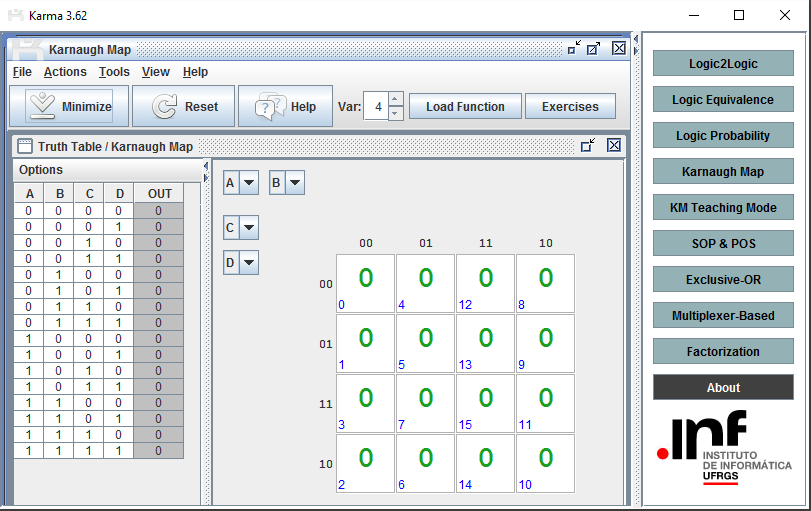
\includegraphics[width=\maxwidth{.95\linewidth}]{gfx/07_02}
	\caption{Karnaugh Map Screen}
	\label{fig:07_02}
\end{figure}

\subsubsection{Data Entry} When using \gls{karma}, the first step is to input some sort of information about the circuit to be analyzed. That information can be entered in several different formats, but the most common for this class would be either a truth table or a Boolean expression.

To enter the initial data, click the Load Function button at the top of the canvas.

By default, the Load Function screen opens with a blank screen. In the lower left corner of the Load Function window, the Source Format for the input data can be selected. There is a template available for each of the different source formats; and that template can be used to help with data entry. The best way to work with \gls{karma} is to click the ``Templates'' button and select the data format being used. In Figure \ref{fig:07_03}, the ``Expression 1'' template was selected:

\begin{figure}[H]
	\centering
	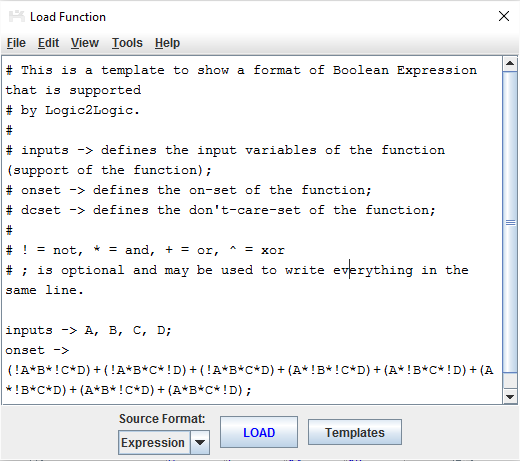
\includegraphics[width=\maxwidth{.95\linewidth}]{gfx/07_03}
	\caption{The Expression 1 Template}
	\label{fig:07_03}
\end{figure}

The designer would replace the ``inputs'' and ``onset'' lines with information for the circuit being simplified. Once the source data are entered into this window, click the ``Load'' button at the bottom of the window to load the data into \gls{karma}.

\subsubsection{Data Source Formats}

Karma works with input data in any of six different formats: Boolean Expression, Truth Table, Integer, Minterms, Berkeley Logic Interchange Format (\textit{BLIF}), and Binary Decision Diagram (\textit{BDD}). \textit{BLIF} and \textit{BDD} are programming tools that are beyond the scope of this lesson and will not be covered.

\paragraph{Expression}

Boolean expressions can be defined in Karma using the following format.

\begin{verbatim}
     #Sample Expression
     (!x1*!x2*!x4)+(!x1*x2*!x3)+(x1*!x4*!x5)+(x1*x3*x4)
\end{verbatim}

Notes:

\begin{itemize}
	\item Any line that starts with a hash tag (``\#'') is a comment and will be ignored by Karma.
	\item ``Not'' is indicated by a leading exclamation mark. Thus ``!x1'' is the same as X1'.
	\item All operations are explicit. In real‐number algebra the phrase ``AB'' is understood to be ``A*B''. However, in \gls{karma}, since variable names can be more than one character long, all operations must be explicitly stated. AND is indicated by an asterisk and OR is indicated by a plus sign.
	\item No space is left between operations.
\end{itemize}

\paragraph{Truth Table}

A truth table can be defined in \gls{karma} using the following format.

\begin{Verbatim}[commandchars=\\\{\}]
     #Sample Truth Table 
     inputs -\textgreater X, Y, Z 
     000 : 1
     001 : 1 
     010 : 0 
     011 : 0 
     100 : 0 
     101 : 1 
     110 : 0 
     111 : 1
\end{Verbatim}

Notes:

\begin{itemize}
	\item Any line that starts with a hash tag (``\#'') is a comment and will be ignored by \gls{karma}.
	\item The various inputs are named before they are used. In the example, there are three inputs: X, Y, and Z.
	\item Each row in the truth table is shown, along with the output required. So, in the example above, an input of 000 should yield an output of 1.
	\item An output of ``-'' is permitted and means ``don't care.''
\end{itemize}

\paragraph{Integer}

In Karma, an integer can be used to define the outputs of the truth table, so it is ``shorthand'' for an entire truth table input. Following is the example of the ``integer'' type input.

\begin{Verbatim}[commandchars=\\\{\}]
     #Sample Integer Input 
     inputs -\textgreater A, B, C, D 
     onset -\textgreater E81A base 16
\end{Verbatim}

Notes:

\begin{itemize}
	\item Any line that starts with a hash mark (``\#'') is a comment and will be ignored by Karma.
	\item Input variables are defined first. In this example, there are four inputs: A, B, C, and D.
	\item The ``onset'' line indicates what combinations of inputs should yield a True on a truth table. 
\end{itemize}

In the example, the number E81A is a hexadecimal number that is written like this in binary:

\begin{verbatim}
     1110 1000 0001 1010 
       E    8    1    A
\end{verbatim}

The least significant bit of the binary number, 0 in this example, corresponds to the output of the first row in the truth table; thus, it is false. Each bit to the left of the least significant bit corresponds to the next row, counting from 0000 to 1111. Following is the truth table generated by the hexadecimal integer E81A.

\begin{table}[H]
	\sffamily
	\newcommand{\head}[1]{\textcolor{white}{\textbf{#1}}}		
	\begin{center}
		\rowcolors{2}{gray!10}{white} % Color every other line a light gray
		\begin{tabular}{ccccc} 
			\rowcolor{black!75}
			\multicolumn{4}{c}{\head{Inputs}} & \head{Output} \\
			A & B & C & D & Q \\
			\hline
			0 & 0 & 0 & 0 & 0 \\
			0 & 0 & 0 & 1 & 1 \\
			0 & 0 & 1 & 0 & 0 \\
			0 & 0 & 1 & 1 & 1 \\
			0 & 1 & 0 & 0 & 1 \\
			0 & 1 & 0 & 1 & 0 \\
			0 & 1 & 1 & 0 & 0 \\
			0 & 1 & 1 & 1 & 0 \\
			1 & 0 & 0 & 0 & 0 \\
			1 & 0 & 0 & 1 & 0 \\
			1 & 0 & 1 & 0 & 0 \\
			1 & 0 & 1 & 1 & 1 \\
			1 & 1 & 0 & 0 & 0 \\
			1 & 1 & 0 & 1 & 1 \\
			1 & 1 & 1 & 0 & 1 \\
			1 & 1 & 1 & 1 & 1 \\
		\end{tabular}
	\end{center}
	\caption{Truth Table for E81A Output}
	\label{tab:e81a_output}
\end{table}

The ``Output'' column contains the binary integer $1110$ $1000$ $0001$ $1010$ (or $E81A$h) from bottom to top.

\paragraph{Terms}

Data input can be defined by using the minterms for the Boolean expression. Following is an example minterm input.

\begin{Verbatim}[commandchars=\\\{\}]
     #Sample Minterms 
     inputs -\textgreater A, B, C, D
     onset -\textgreater 0, 1, 2, 3, 5, 10
\end{Verbatim}

Notes:

\begin{itemize}
	\item Any line that starts with a hash mark (``\#'') is a comment and will be ignored by \gls{karma}.
	\item The inputs, A, B, C, and D, are defined first.
	\item The ``onset'' line indicates the minterms that yield a ``true'' output.
	\item This is similar to a SOP Sigma expression, and the digits in that expression could be directly entered on the onset line. For example, the onset line above would have been generated from this Sigma expression:

	$ \int(A,B,C,D)=\sum(0,1,2,3,5,10) $
\end{itemize}

\subsubsection{Truth Table and Karnaugh Map Input}

While Karma will accept a number of different input methods, as described above, one of the easiest to use is the Truth Table and its related Karnaugh Map, and these are displayed by default when the \textit{Karnaugh Map} function is selected. The value of any of the cells in the \textit{Out} column in the Truth Table, or cells in the Karnaugh Map, and can be cycled through 0, 1, and ``don’t care'' (indicated by a dash) on each click of the mouse in the cell. The Truth Table and Karnaugh Map are synchronized as cells are clicked. The number of input variables can be adjusted by changing the \textit{Var} setting at the top of the screen. Also, the placement of those variables on the Karnaugh Map can be adjusted as desired.

\subsubsection{Solution}

To simplify the Karnaugh Map, click the Minimize button. A number of windows will pop up (illustrated in Figure \ref{fig:07_04}), each showing the circuit simplification in a slightly different way. Note: this Boolean expression was entered to generate the following illustrations: $ A'C + A'B + AB'C' + B'C'D' $. 

\begin{figure}[H]
	\centering
	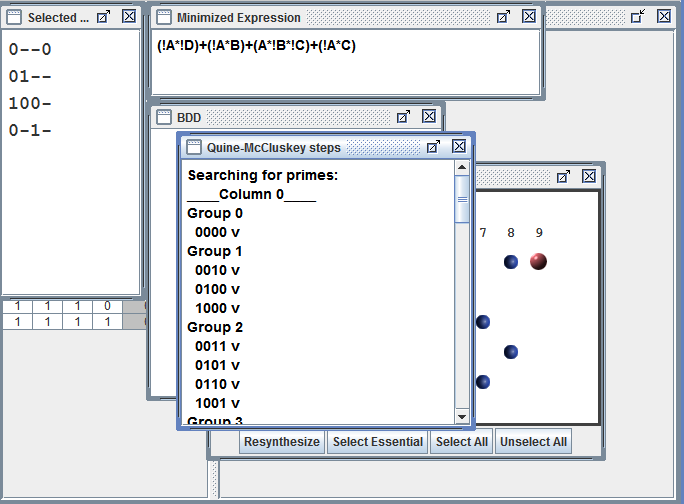
\includegraphics[width=\maxwidth{.95\linewidth}]{gfx/07_04}
	\caption{A KARMA Solution}
	\label{fig:07_04}
\end{figure}

\paragraph{Boolean Expression}

The minimized Boolean expression is shown in Figure \ref{fig:07_05}.

\begin{figure}[H]
	\centering
	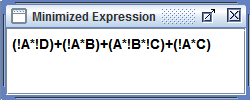
\includegraphics[width=\maxwidth{.95\linewidth}]{gfx/07_05}
	\caption{The Minimized Boolean Expression}
	\label{fig:07_05}
\end{figure}

In this solution, a NOT term is identified by a leading exclamation point; thus, the minimized expression is: $ A'D' + AB'C' + A'C + A'B $.

\paragraph{BDDeiro}

The \textit{BDDeiro} window is a form of Binary Decision Diagram (\textit{BDD}). The decision tree for the minimized expression is represented graphically in Figure \ref{fig:07_06}.

\begin{figure}[H]
	\centering
	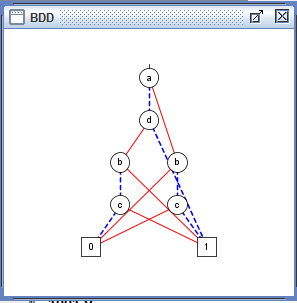
\includegraphics[width=\maxwidth{.95\linewidth}]{gfx/07_06}
	\caption{The BDDeiro Solution}
	\label{fig:07_06}
\end{figure}

The top node represents input \textit{a}, which can either be true or false. If false, then follow the blue dotted line down to node \textit{d}, which can also be either true or false. If \textit{d} is false, follow the blue dotted line down to the \textit{1} output. This would mean that one True output for this circuit is $ A'D' $, which can be verified as one of the outputs in the minimized expression.

Starting at the top again, if \textit{a} is true, then follow the solid red line down to \textit{b}. It that is true, then follow the red solid line down to the \textit{0} output. The expression $ AB $ is false and does not appear in the minimized solution. In a similar way, all four True outputs, and three false outputs, can be traced from the top to bottom of the diagram.

\paragraph{Quine-McCluskey}

Karma includes complete Quine‐McCluskey solution data. Several tables display the various implicants and show how they are derived.

\begin{figure}[H]
	\centering
	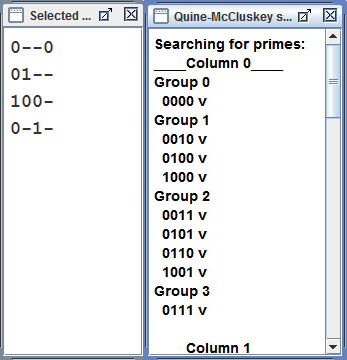
\includegraphics[width=\maxwidth{.95\linewidth}]{gfx/07_07}
	\caption{Quine-McCluskey Solution}
	\label{fig:07_07}
\end{figure}

Karma also displays the Covering Table for a Quine‐McCluskey solution. Each of the minterms (down the left column) can be turned on or off by clicking on it. The smaller blue balls in the table indicate prime implicants and the larger red balls (if any) indicate essential prime implicants. Because this table is interactive, various different solutions can be attempted by clicking some of the colored markers to achieve the best possible simplification.

\begin{figure}[H]
	\centering
	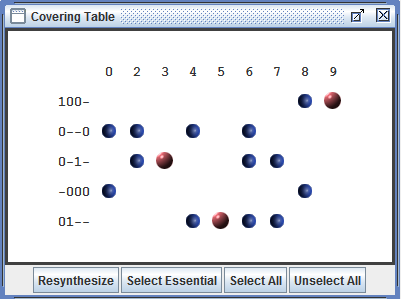
\includegraphics[width=\maxwidth{.95\linewidth}]{gfx/07_08}
	\caption{Selecting Implicants}
	\label{fig:07_08}
\end{figure}

\subsubsection{Practice Problems}

The following problems are presented as practice for usingKarma to simplify a Boolean expression. Note: designers can select different Prime Implicants so the simplified expression could vary from what is presented below.

\begin{table}[H]
	\sffamily
	\begin{center}
		\begin{tabular}{c c p{8cm} }
			\multirow{2}{*}{\textbf{1}} 
			& Expression & $ \int(A,B,C,D) = \sum(5,6,7,9,10,11,13,14) $ \\
			& \cellcolor{gray!10} Simplified 
			& \cellcolor{gray!10} $ BC'D+A'BC+ACD'+AB'D $ \\
			\hline
			\multirow{2}{*}{\textbf{2}} 
			& Exression & $ A'BC'D+A'BCD'+A'BCD+AB'C'D+AB'CD'+AB'CD+AB'CD+ABC'D+ABCD' $ \\
			& \cellcolor{gray!10} Simplified 
			& \cellcolor{gray!10} $ BC'D+A'BC+ACD'+AB'D $ \\
			\hline
			\multirow{2}{*}{\textbf{3}} 
			& Exression & 4-variable Karnaugh Map where cells 5,6,7,9,10 are True and 13,14 are Don't Care  \\
			& \cellcolor{gray!10} Simplified 
			& \cellcolor{gray!10} $ BC'D+AC'D+A'BC+ACD' $ \\
			\hline
			\multirow{2}{*}{\textbf{3}} 
			& Exression & $ \int(A,B,C,D,E) = \sum(0,3,4,12,13,14,15,24,25,28,29,30) $ \\
			& \cellcolor{gray!10} Simplified 
			& \cellcolor{gray!10} $ ABD'+A'B'C'DE+BCE'+A'BC+A'B'D'E' $ \\
		\end{tabular}
	\end{center}
	\caption{KARMA Practice Problems}
	\label{tab:karma_practice_problems}
\end{table}













%%%%%%%%%%%%%%%%%%%%%%%%%%%%%%%%%%%%%%%%%%%%%%%%%%%%%%%%%%%%%%%%%%%%%

\subsection{32x8}

One online site of interest is \url{http://www.32x8.com/}. This site permits visitors to set up a truth table with two to eight variables and then will create a simplified Boolean circuit for that truth table.

